\documentclass{standalone}
\usepackage{tikz}
\usetikzlibrary{shapes.geometric, arrows}

\tikzstyle{startstop} = [ellipse, minimum width=3cm, minimum height=1cm, text centered, draw=black, fill=red!30]
\tikzstyle{process} = [rectangle, minimum width=3cm, minimum height=1cm, text centered, draw=black, fill=orange!30]
\tikzstyle{arrow} = [thick,->,>=stealth]

\begin{document}

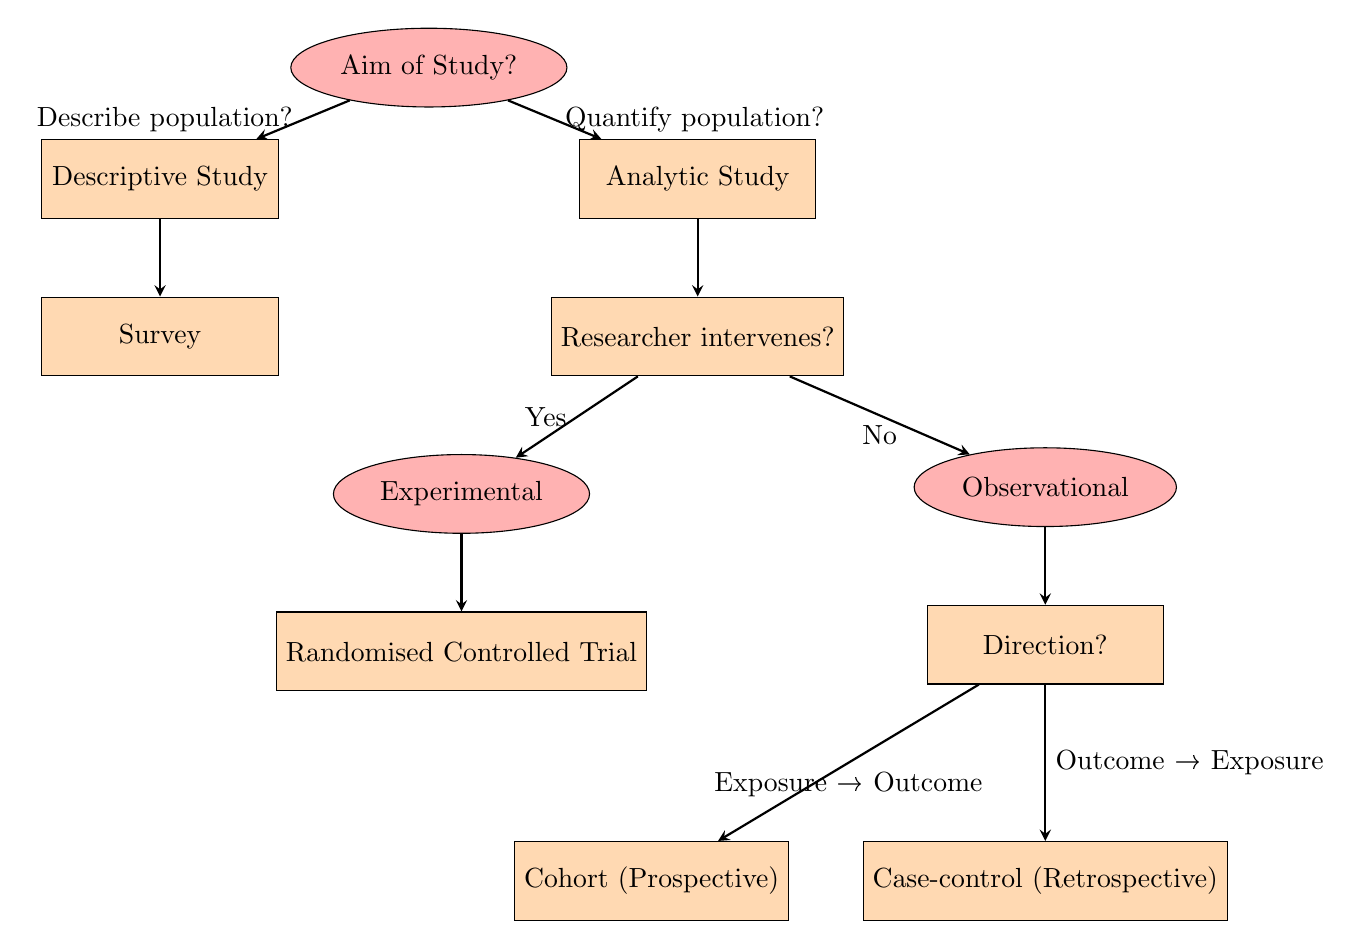
\begin{tikzpicture}[node distance=2cm]

\node (study) [startstop] {Aim of Study?};
\node (desc) [process, below left of=study, xshift=-2cm] {Descriptive Study};
\node (analytic) [process, below right of=study, xshift=2cm] {Analytic Study};
\node (survey) [process, below of=desc] {Survey};
\node (inter) [process, below of=analytic] {Researcher intervenes?};
\node (exp) [startstop, below of=inter, xshift=-3cm] {Experimental};
\node (obs) [startstop, below right of=inter, xshift=3cm, yshift=-0.5cm] {Observational};
\node (rct) [process, below of=exp] {Randomised Controlled Trial};
\node (dir) [process, below of=obs] {Direction?};
\node (cohort) [process, below of=dir, yshift=-1cm] {Case-control (Retrospective)};
\node (casecontrol) [process, left of=cohort, xshift=-3cm] {Cohort (Prospective)};

\draw [arrow] (study) -- node[anchor=east] {Describe population?}(desc);
\draw [arrow] (study) -- node[anchor=west] {Quantify population?}(analytic);
\draw [arrow] (desc) -- (survey);
\draw [arrow] (analytic) -- (inter);
\draw [arrow] (inter) -- node[anchor=east] {Yes} (exp);
\draw [arrow] (inter) -- node[anchor=north] {No} (obs);
\draw [arrow] (exp) -- (rct);
\draw [arrow] (obs) -- (dir);
\draw [arrow] (dir) -- node[anchor=west] {Outcome → Exposure} (cohort);
\draw [arrow] (dir) -- node[anchor=north] {Exposure → Outcome} (casecontrol);

\end{tikzpicture}

\end{document}
